\chapter{绪论}
\section{数据中心网络}
现代数据中心在共享的设备资源基础上,为多个用户提供不同的服务。
为保障数据安全以及用户的独立性,数据中心向每个用户展现的是虚拟化的网络环境。
这就需要数据中心的管理者部署灵活的网络功能来实现这一要求。

由于硬件网络设备普遍灵活性受限,几乎所有的云服务商都用软件来实现其网络功能,
例如:微软、亚马逊、VMWare等\cite{azure, 179731}。但软件实现网络功能的性能天然存在两个问题:

其一,吞吐率受限。现有的软件定义网络功能通常需要使用两个以上核才能达到10Gbps带宽
\cite{Martins:2014:CAN:2616448.2616491,180672},
而最新的网络设备带宽已达到40\textasciitilde 100Gbps\cite{edr}。
尽管增加单服务器的核数能够提升部分性能,但与此同时成本也会大幅提升。
一方面是设备开销提高,另一方面则是能耗显著增加。

其二,延迟高且不稳定。现有软件定义网络的处理延迟从几十微秒到毫秒量级不等
\cite{Gandhi:2014:DCS:2619239.2626317, Martins:2014:CAN:2616448.2616491, Gandhi:2014:DCS:2619239.2626317}。
无法满足证券交易等对低延迟要求严苛的应用需求。

在图形处理器(graphics processing unit, GPU)\cite{Han:2010:PGS:1851275.1851207}、
专用网络处理器\cite{cavium, netronome}和FPGA\cite{sigcomm2015keynote, Naous:2008:NRR:1397718.1397720}
上均有相关的工作旨在保障灵活性的基础上克服软件处理网络包的上述限制。
相比于GPU而言,FPGA能耗更低\cite{5681761, 5572788};相比于专用网络处理器,FPGA可通过硬件逻辑实现更多服务所需的功能。
更重要的是,将FPGA部署在大规模数据中心的成本更低\cite{sigcomm2015keynote,6853195}。

在数据中心中利用FPGA加速软件网络功能从预期上能够达到较好的性能,
但实践中面临的主要问题是编程方面困难。传统的FPGA逻辑是通过Verilog、VHDL等硬件描述语言编写,
这些语言所展现的是门、寄存器、多路选择器、时钟等非常底层的器件。
这样虽然方便手工优化逻辑,但也导致编程复杂度高、开发效率低下、调试方面等问题。
这些困难导致多年来很多人远离FPGA编程\cite{Bacon:2013:FPM:2436256.2436271}。

本文借助微软亚洲研究院无线与网络研究组最新开发的ClickNP平台\cite{clicknp}进行FPGA编程,
针对数据中心网络场景优化了包生成器及抓包器、OpenFlow防火墙、IPSec网关、L4负载均衡、pFabric流调度器等应用,
并对其性能进行评测。

\section{场效可编程门阵列体系结构}
场效可编程门阵列(FPGA)由大量逻辑门组成。其基本编程单元为逻辑块,由查找表和寄存器组成。
其中查找表可编程为任何组合逻辑计算,寄存器可以存储状态。
FPGA还包含存储数据的块随机访问存储器(block random access memory)、
处理复杂算术运算的数字信号处理单元(digital signal processing)。
FPGA通过PCIe子板与主机相连,其中子板包含数G字节的动态随机访问存储器(dynamic random access memory)
以及10G/40G以太网端口等其他通信界面。

相比于CPU和GPU而言,FPGA的时钟频率较低、访存带宽较小。
典型的FPGA时钟频率在200MHz左右,相比于时钟频率2\textasciitilde 3GHz的CPU低一个多数量级。
FPGA到单个块存储器和外部的动态存储器的带宽约为2\textasciitilde 4GBps,
而英特尔至强处理器的访存带宽约为40GBps,GPU的带宽则高达100GBps。

但相比于被有限核数限制并行数的CPU和GPU而言,FPGA的可并行化程度较高。
现代的FPGA可以集成数百万个逻辑块、数百Kbit寄存器、数十Mbit块存储器以及数千个数字信号处理单元。
理论上,所有这些器件均可并行地工作。因此数千个“核”在同一个FPGA芯片中并行工作是有可能的。
尽管单个块存储器的带宽有限,但同时访问数千个块存储器可使带宽达到TBps量级。
因此,为了在FPGA平台上实现高性能,必须充分利用其并行化的能力。

传统的FPGA编程使用Verilog、VHDL等硬件描述语言实现。这些语言关注底层细节,难于学习,编程复杂。

为了减轻编程负担,工业界与学术界均有开发高级编程工具,将以C语言为主的高级语言编写的程序转化为硬件程序。
其中包括微软亚洲研究院无线与网络研究组开发的ClickNP编程平台\cite{clicknp}。

\section{RoCEv2远程直接数据存取协议}
\subsection{直接数据存取}
直接数据存取 (direct memory access, DMA) 是现代计算机系统中常见的访存方式,
这种方式使外围设备可以不经CPU而直接访问存储器。

在非DMA访存模式下,CPU采用可编程输入输出方式与外围设备进行数据交互。
在等待设备完成读写操作期间,CPU无法处理其他任务,这一停等浪费大量计算资源。

在DMA访存模式下,CPU将数据传输初始化,在随后的数据传输过程中处理其他任务。
在数据传输结束时,会从DMA控制器收到表明操作完成的中断。
这一特性既适用于数据传输率远高于CPU处理能力的情况,
也适用于需要CPU利用等待时间处理更重要任务的情况。

\subsection{远程直接数据存取}
远程直接数据存取 (remote direct memory access, RDMA) 是不经过任何一台设备上操作系统的设备间访存方式。

RDMA设备接收到特定的数据包之后不再交由操作系统处理,而直接根据其请求访问本地存储器并进行反馈。
而CPU只负责初始化和结束RDMA设备,在数据传输过程中不会收到中断请求。

\subsection{RoCE协议}
基于融合以太网络的RDMA (RDMA over Converged Ethernet, RoCE) 协议允许设备间通过以太网络进行远程直接内存访问。
该协议由两个版本,分别称为RoCEv1和RoCEv2。其中RoCEv1将以太网协议作为其链路层该协议,
因而允许在同一个以太网广播域下的任意两台主机间进行通信\cite{a16}。
RoCEv2则基于用户数据报协议 (user datagram protocol, UDP),因而可以经过路由\cite{a17, considerations, storage}。

\begin{figure}[htbp]
\centering
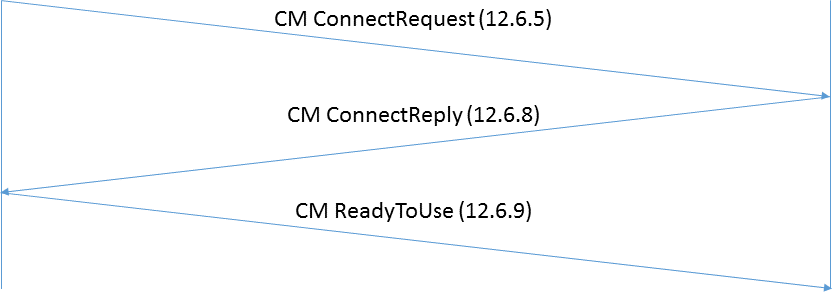
\includegraphics[width=4in]{rocereq}
\caption{建立RoCE连接} \label{fig:rocereq}
\end{figure}

\begin{figure}[htbp]
\centering
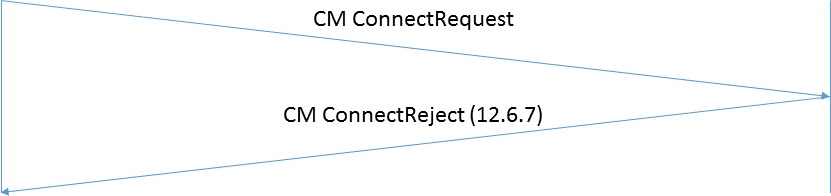
\includegraphics[width=4in]{rocerej}
\caption{建立RoCE连接被拒绝} \label{fig:rocerej}
\end{figure}

\begin{figure}[htbp]
\centering
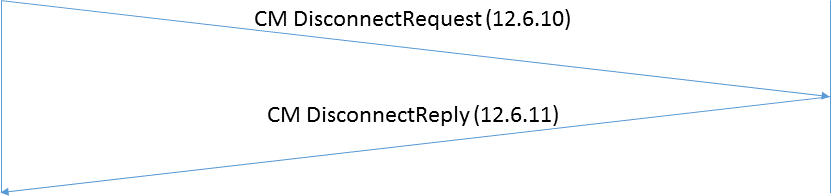
\includegraphics[width=4in]{rocedreq}
\caption{断开RoCE连接} \label{fig:rocedreq}
\end{figure}

\begin{figure}[htbp]
\centering
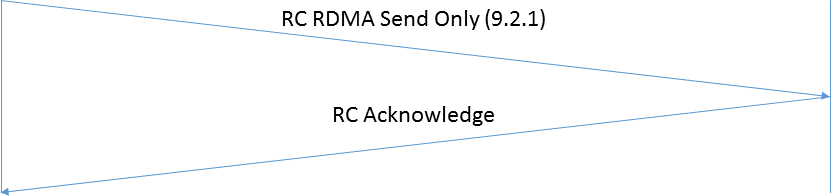
\includegraphics[width=4in]{rocewriteonly}
\caption{单RoCE包写操作} \label{fig:rocewriteonly}
\note{在数据载荷不多于1024字节时的写请求只包含单包,数据发送请求的工作过程与之类似。}
\end{figure}

\begin{figure}[htbp]
\centering
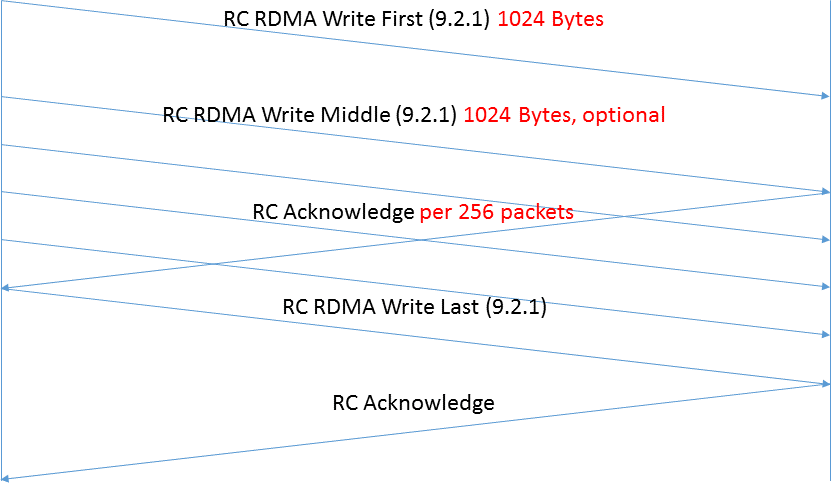
\includegraphics[width=4in]{rocewritemany}
\caption{多RoCE包写操作} \label{fig:rocewritemany}
\note{对于超过1024字节的数据载荷,先后发送Write First、Write Middle (如有)、Write Last三种包。
自Write First起,接收端每收到256个包反馈一个确认包,也对最后一个包进行反馈,
数据发送请求的工作过程与之类似。}
\end{figure}

\begin{figure}[htbp]
\centering
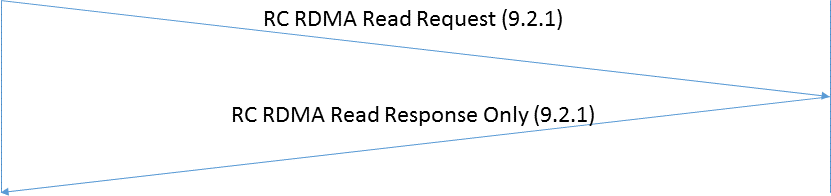
\includegraphics[width=4in]{rocereadonly}
\caption{单RoCE包读操作} \label{fig:rocereadonly}
\note{在数据载荷不多于1024字节时读响应至包含单包}
\end{figure}

\begin{figure}[htbp]
\centering
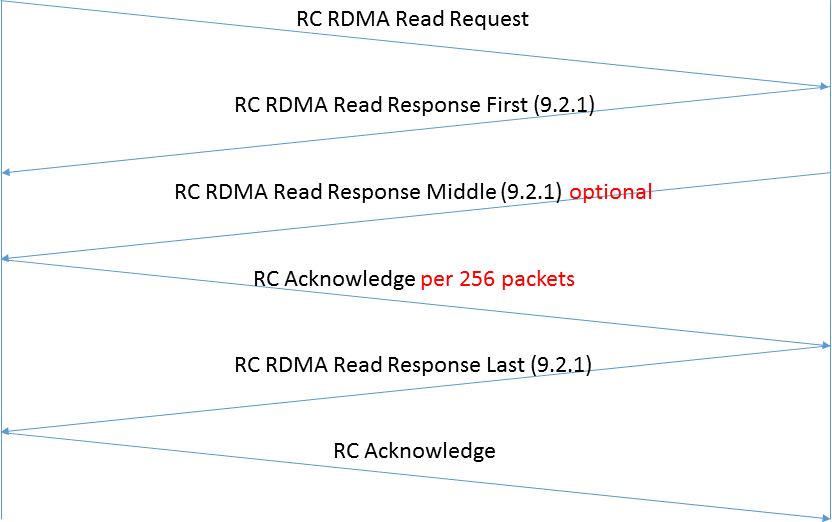
\includegraphics[width=4in]{rocereadmany}
\caption{多RoCE包读操作} \label{fig:rocereadmany}
\note{对于超过1024字节的数据载荷,先后发送Read Response First、Read Response Middle (如有)、
Read Response Last三种包。自Read Response First起,接收端没收到256个包反馈一个确认包,
也对最后一个包进行反馈。}
\end{figure}

用户可通过RoCE协议发起读数据、写数据、发送数据三种请求。
其工作过程如图~\ref{fig:rocereq}、图~\ref{fig:rocerej}、图~\ref{fig:rocedreq}、
图~\ref{fig:rocewriteonly}、图~\ref{fig:rocewritemany}、图~\ref{fig:rocereadonly}所示。

面对网络中可能出现的丢包情况,RoCE协议具有与TCP/IP类似的重传策略:
对每个消息赋予一个包序列号。如果接收端收到的包序列号不连续,则反馈缺失消息,
并提供缺失的第一个包序列号。发送端从该序列号对应的包开始重传,如图~\ref{fig:rocewritenak} 所示。
\begin{figure}[htbp]
\centering
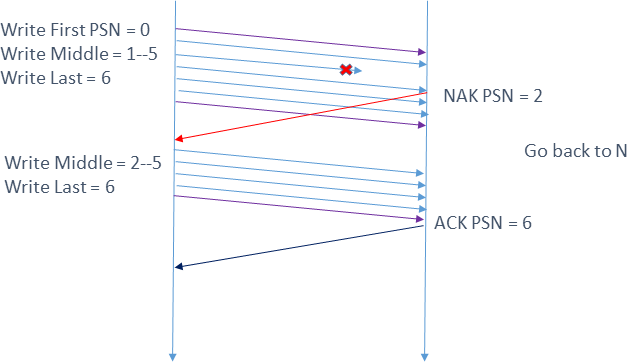
\includegraphics[width=4in]{rocewritenak}
\caption{RoCE重传策略} \label{fig:rocewritenak}
\end{figure}

